%!TEX root = ../dissertation.tex

\begin{savequote}[75mm]
Another inspiring quote for this chapter
\qauthor{Another author maybe}
\end{savequote}


\chapter[High-performance computing in healthcare: An automatic literature analysis perspective]{High-performance computing in healthcare: An automatic literature analysis perspective}

\lettrine[lines=3]{\textcolor{SchoolColor}{T}}{%bstract of the chapter could go here
}
he adoption of high-performance computing (HPC) in healthcare has gained significant attention in recent years, driving advancements in medical research and clinical practice. Exploring the literature on HPC implementation in healthcare is valuable for decision-makers as it provides insights into potential areas for further investigation and investment. However, manually analyzing the vast number of scholarly articles is a challenging and time-consuming task. Fortunately, topic modeling techniques offer the capacity to process extensive volumes of scientific literature, identifying key trends within the field. This paper presents an automatic literature analysis framework based on a state-of-art vector-based topic modeling algorithm with multi-embedding techniques, unveiling the research trends surrounding HPC utilization in healthcare. The proposed pipeline consists of four phases: paper extraction, data preprocessing, topic modeling and outlier detection, followed by visualization. It enables the automatic extraction of meaningful topics, exploration of their interrelationships, and identification of emerging research directions in an intuitive manner. The findings highlight the transition of HPC adoption in healthcare from traditional numerical simulation and surgical visualization to emerging topics such as drug discovery, AI-driven medical image analysis, and genomic analysis, as well as correlations and interdisciplinary connections among application domains.

\section{Introduction}\label{se:2-1}

High Performance Computing (HPC) is increasingly becoming an indispensable resource in healthcare research due to its capabilities in addressing complex and data-intensive tasks~\cite{elsebakhi2015large,raj2015big,jia2014gpu}. The exponential growth of health data next to simulation and modeling drives the adoption of HPC, which encompasses i.a., genomic sequencing, biomedical imaging, electronic health records (EHRs), and wearable device data \cite{bastrakov2013high,schmidt2017next,stocker2010high,alanazi2015meeting,vitabile2019medical}. Effectively managing and analyzing such data poses significant challenges in storage, management, and analysis, necessitating the computational power offered by HPC. In genomics, HPC allows researchers to analyze genomic data at a scale and speed previously impossible, revealing genetic bases of various diseases and helping develop personalized treatments~\cite{molidor2003new,lightbody2019review}. Similarly, HPC plays a crucial role in drug discovery and computational modeling  \cite{CHEN20181241,jumper2021highly}.
Drug discovery processes are traditionally time and resource-intensive. However, HPC allows researchers to conduct molecular dynamics simulations to understand drug-protein interactions at the atomic level, speeding up the process and reducing costs~\cite{zhang2014toward,ge2013molecular,sanbonmatsu2007high}. Furthermore, HPC-enabled computational modeling allows the simulation of biological systems or disease progression, providing insights to inform treatment strategies~\cite{kharche2008simulation,perrin2010model}. The deployment of HPC in Artificial Intelligence (AI) for healthcare has also experienced substantial growth. HPC enables the implementation of advanced AI techniques, which necessitate substantial computational power to efficiently handle extensive data volumes and complex deep neural networks~\cite{phong2017brain,cirillo2019big}. Biomedical imaging stands as a prime example where HPC assumes a crucial role \cite{LITJENS201760}. By leveraging HPC, AI tools can swiftly process and analyze high-resolution images, facilitating real-time analysis of complex imaging data and leading to expedited and more precise diagnoses~\cite{cai2020review,tahmassebi2018deep}. In addition, HPC-enabled convergence of AI and simulation has significantly improved the quality and speed of traditional simulation in healthcare~\cite{lee2019deepdrivemd,bai2022application}. 

Investigating the literature on HPC adoption in healthcare can generate valuable insights that are beneficial for the business and economic side of healthcare by providing a comprehensive understanding of the current landscape and potential future directions. These insights can guide strategic planning and investment decisions of HPC in healthcare businesses, highlighting promising areas for further exploration and development. However, the substantial volume of literature, combined with the rapid pace of technological advancements, makes manual analysis very difficult and time consuming. As a result, there is a recognized need for an automated literature analysis framework to accurately process the vast corpus of literature, transforming it into meaningful insights for business or strategic decision making within the healthcare sectors.

Topic modeling, a family of typically unsupervised machine learning approaches, aims at discovering hidden semantic structures, or `topics', within a corpus of text~\cite{blei2012probabilistic}. The underlying principle of topic modeling is to classify text documents into different topics based on the frequency and co-occurrence of words~\cite{jacobi2018quantitative}. The strength of topic modeling lies in its capacity to handle large and unstructured datasets, rendering it an invaluable tool for exploratory data analysis. Prominent techniques employed in topic modeling include Latent Dirichlet Allocation (LDA)~\cite{blei2003latent}, Non-negative Matrix Factorization (NMF)~\cite{lee1999learning}, and Latent Semantic Analysis (LSA)~\cite{deerwester1990indexing}. With a broad range of applications in areas such as text mining, information retrieval, and digital humanities, topic modeling continues to garner considerable interest~\cite{alghamdi2015survey,yi2009comparative,meeks2012digital}. Topic modeling has become an increasingly popular tool in scientific research and literature review~\cite{asmussen2019smart,amado2018research,chen2019identify}. Its usage spans various scientific research fields, including marketing, medical, and social sciences~\cite{amado2018research,algaa2020analysis,lindstedt2019structural}. In the context of literature reviews, topic modeling has been used to identify trends and patterns in large bodies of literature. For instance, it has been used to analyze collective behavior and social movements by sociologists~\cite{lindstedt2019structural}, and also been adopted to understand the big data themes from biomedical research~\cite{van2016understanding}. 

LDA is arguably one of the most widely used algorithms for topic modeling. However, it has been characterized by certain constraints, including the prerequisite of data cleaning and pre-processing, the requirement to specify model parameters such as $\alpha$ (document-topic density), $\beta$ (topic-word density) and topic numbers hyperparameters. Moreover, the challenges associated with the interpretability and validation of the generated topics also need to be addressed~\cite{maier2018applying,angelov2020top2vec}, which is why alternatives such as entity linking (EL) have been frequently deployed, especially in case of shorter texts \cite{10.1145/3126686.3126776}. In response to these limitations, recently developed deep learning algorithms such as Top2Vec, offer alternative approaches for topic modeling~\cite{angelov2020top2vec}. Top2Vec transforms each word in a text collection into a vector representation within a semantic space using an encoding model such as doc2vec or state of the art transformers. Consequently, it autonomously identifies topics within the text and generates jointly embedded topic, document, and word vectors. Comparative studies between LDA and Top2Vec have been conducted, revealing that Top2Vec tends to yield qualitatively superior results compared to LDA~\cite{egger2022topic,karas2022experiments}.

In this study, we propose an automatic literature analysis framework, using a complex question of the impact of HPC on healthcare as the test-bed. The primary contributions of this work are twofold:

\begin{enumerate}
\item We present an automatic literature analysis framework, from document (i.e. scientific article) retrieval and analysis to various interactive visualizations to depict research trends, topics evolution, interconnection across research areas and high impact papers. This adaptable pipeline can be easily applied to other domains by modifying the initial query keywords.
\item By deploying the automated literature analysis framework, we investigate the research trends of HPC utilization in healthcare. Our analysis reveals notable shifts in research focus, spanning from visualization and rendering in surgical practice and traditional numerical simulation to emerging topics such as drug discovery, AI-driven medical image analysis, and genomic analysis. These insights provide valuable indications for future investment and strategic development of HPC within the healthcare sector, guiding decision-making and resource allocation.
\end{enumerate}

\section{Materials and methods}\label{se:2-2}

In this section, we provide a comprehensive description of the data and analysis process employed in our study. Figure~\ref{fig:2-1} illustrates the automatic literature review framework implemented in our study, which consists of four distinct stages: paper retrieval and extraction, data preprocessing, topic modeling, and visualization. The subsequent sections provide detailed explanations of each stage.
\begin{figure}[!h]
\centering
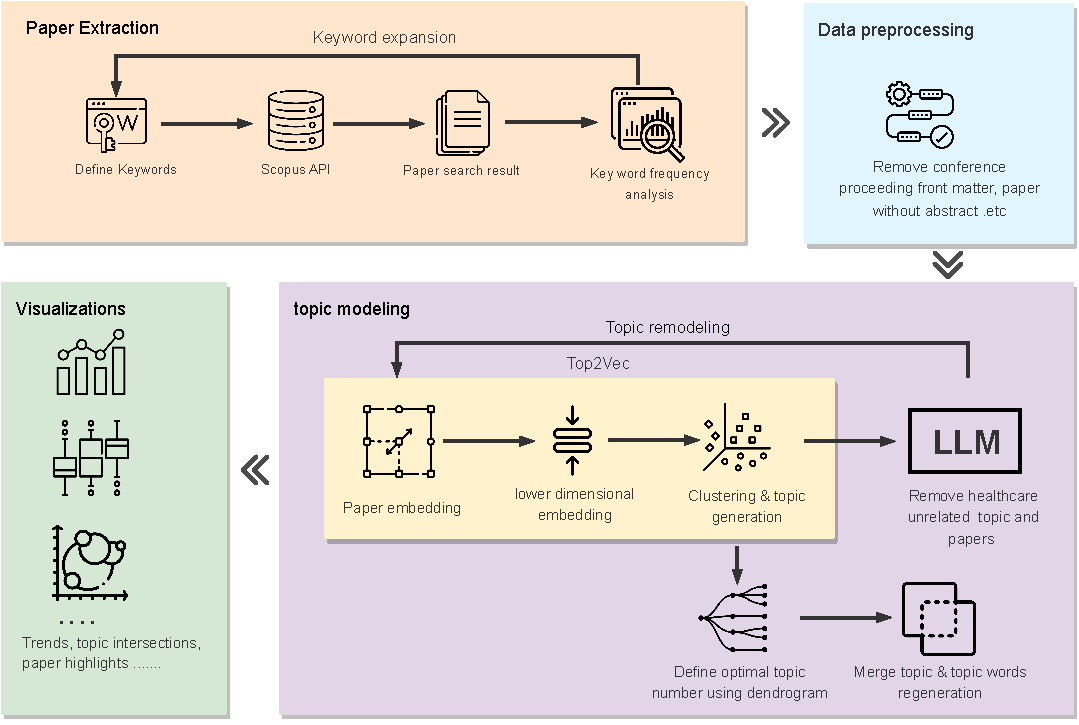
\includegraphics[width=0.9\textwidth]{2-1.pdf}
\caption{Automatic literature review pipeline consists of four stages: paper retrieval and extraction, data preprocessing, topic modeling, and visualization}
\label{fig:2-1}
\end{figure}


\subsection{Paper retrieval and extraction}\label{subse:2-2.1}
\subsubsection{Data source}\label{subsubse:2-2.1.1}

Scopus\footnote{\url{https://www.elsevier.com/solutions/scopus}}  has been utilized in our study as it is the largest publicly available abstract and citation database of peer-reviewed literature, including scientific journals, books and conference proceedings.

\subsubsection{Type of articles included in the study}\label{subsubse:2-2.1.2}

In this study, conference papers, journal papers, books or book chapters, editorial materials, early access workshop papers and presentations published in English are included. Conference proceeding front matters, meeting abstracts, errata and papers without abstracts are excluded from the analysis. Since the publication year 2023 is not yet complete, studying trends beyond 2022 may introduce bias. Therefore, we limit our analysis to publications up until end of 2022.



\subsubsection{Paper retrieval pipeline}\label{subsubse:2-2.1.3}

We establish an automatic paper record retrieval and query expansion pipeline through the Scopus API\footnote{\url{https://dev.elsevier.com/}}. During the initial phase of query construction, we take into account the co-occurrence of HPC keywords such as `high performance computing' and `supercomputing' along with the most prevalent health-related terms like `healthcare', `health', `clinic',`medicine', `disease', and `treatment'. With each iteration of the literature search, we implement query expansion by incorporating additional relevant keywords extracted from the retrieved scientific paper documents. To achieve this, we perform a frequency analysis of keywords extracted from the titles and abstracts. Keywords that are identified as HPC or healthcare-related and occur with a frequency of 50 or higher, but are not previously included, are considered as new keywords and subsequently added to the expanded query. Such automatic query expansion process results in inclusion of the synonyms of HPC, such as `high-performance computing', `high performance computer', and `supercomputer', along with broader or narrower healthcare-related terms like `patient', `diagnosis', `drug', `therapy', `pharmaceutical', `surgery', and others. This process is repeated until no new keywords emerge, indicating the completion of the search query expansion. The extracted literature serves as an input for further processing in the subsequent steps.


\subsection{Data preprocessing}\label{subse:2-2.2}
Based on the output obtained from Scopus, we retain the title, abstract, publication date, and citation number for subsequent topic modeling and visualization. Given that the Top2Vec algorithm does not require stop-word lists nor stemming, or lemmatization, the title and abstract of each literature piece are merged as the model input without further preprocessing.
\subsection{Topic Modeling }\label{subse:2-2.3}

\subsubsection{Algorithm choice}\label{subsubse:2-2.3.1}

We adopt the Top2Vec model for topic modeling, an innovative unsupervised machine learning algorithm designed for automatic topic detection and document embedding~\cite{angelov2020top2vec}. This model is unique as it combines the strengths of word embeddings, dimensionality reduction, and density-based clustering to identify topics from a given set of documents without any prior knowledge or human intervention.

The first step in the Top2Vec algorithm involves transforming the documents into dense vector representations using chosen embedding algorithm to capture the semantic meanings of the documents, including the context in which words are used, and represents them as high-dimensional vectors. This process results in a document embedding space where semantically similar documents are located close to each other. We process the input literature by employing five distinct embedding techniques available in the Top2Vec algorithm to generate combined document and word vectors. These techniques include doc2vec~\cite{le2014distributed}, two Universal Sentence Encoder models~\cite{cer2018universal,yang2019multilingual}, and two BERT models~\cite{reimers2019sentence,reimers2020making}. We implement the CV coherence score in our topic modeling evaluation, a metric initially introduced by R?der et al. in their comprehensive examination of coherence measures for topic modeling algorithms~\cite{roder2015exploring}. The CV coherence score combines cosine similarity with Normalized Pointwise Mutual Information (NPMI). This selection is premised on the strong correlation that the CV coherence score maintains with human ratings, outperforming other evaluative measures. Consequently, we choose the embedding model demonstrating the highest CV coherence score for our study. 

Once the documents are represented as vectors, the Top2Vec model applies the UMAP (Uniform Manifold Approximation and Projection) algorithm to reduce the dimensionality of these vectors~\cite{mcinnes1802umap}. UMAP is a manifold learning technique used for dimension reduction. It preserves both the local and global structure of the data, meaning that it maintains the distances between nearby points (local structure) and distant points (global structure). This results in a lower-dimensional space where clusters of document vectors represent unique topics. 

Following the dimensionality reduction, the model uses HDBSCAN (Hierarchical Density-Based Spatial Clustering of Applications with Noise), a density-based clustering algorithm, to identify these clusters~\cite{campello2013density}. HDBSCAN works by finding regions of the reduced space where there are higher densities of document vectors, and it groups these together as clusters. Each cluster represents a unique topic in the document set and the centroid of each cluster is identified as a `topic vector'. This topic vector is a point in the reduced space that best represents the semantic meaning of each topic. The topic vectors are then transformed back into the word space to provide interpretable topics. This is done by finding the words that are most similar to each topic vector, which are then used as the keywords for the topic. One of the key advantages of the Top2Vec model is that it automatically determines the optimal number of topics based on the data. Additionally, it provides both the keywords for each topic and the documents that are most semantically similar to each topic, offering a comprehensive understanding of the topics present in the document set.


\subsubsection{Identify outlier topics not focusing on HPC adoption in healthcare and remodeling}\label{subsubse:2-2.3.2}
During the literature extraction process, articles that contain healthcare and high-performance related keywords within the title, abstract, or keyword sections are extracted via the Scopus API. However, initial topic modeling results reveal that certain articles do not relate to HPC adoption in healthcare. This discrepancy can be attributed to multiple factors. Firstly, while some articles include the terms `high performance computing' and `health' or `healthcare' in their titles or abstracts, they predominantly address aspects of system health such as fault tolerance, job scheduling, and interconnection, rather than human health. This results in these articles being categorized under topics such as system architecture or networks. Secondly, many abstracts begin with a broad statement, such as ``high-performance computing has been widely used in several industries, including healthcare ...'' but the remainder of the abstract primarily discusses the adoption of HPC in domains other than healthcare. 

The GPT-3 series model has demonstrated promising results in binary semantic text classification~\cite{zografos2023gpt}. To fully automate our analysis pipeline and minimize potential bias from human judgment, we employed \texttt{text-davinci-003}, the most advanced model in the GPT-3 series, for non-healthcare related topic detection. Similar to studies~\cite{carpenter2023using,bommarito2022gpt}, following the first round of topic modeling that generates keywords, we design prompts using \texttt{the text-davinci-003} text completion API\footnote[2]{https://platform.openai.com/docs/models/gpt-3-5}. These prompts incorporate the top 20 keywords from each topic, aiming to produce binary outputs that determine whether the keyword combination for each topic pertains to the healthcare domain. To align with our expectation of binary output (\texttt{Yes} or \texttt{No}), we adjust the \texttt{max\_tokens} parameter indicating the upper limit of tokens to be generated, to a smaller value of 5. The \texttt{temperature}  parameter is set to 0 to limit the randomness of the generated responses, ensuring a more focused and deterministic output.  All other hyperparameters are retained at their default values. If a topic is classified as unrelated to healthcare, the articles under that topic are identified as outliers and removed from the dataset. Once all topic keywords have been examined, the remaining literature proceed to the second round of topic modeling.

\subsubsection{Identify optimal topic number using dendrogram}\label{subsubse:2-2.3.3}

Upon evaluating the preliminary output from the Top2Vec model after the outlier detection phase, we observe that certain topics demonstrate substantial similarity and an increased granularity. Examples include multiple themes associated with virus and epidemic research, genomic research, and drug discovery (cf. Section \ref{subse:2-3.2} and Figure~\ref{fig:2-2} for detailed observations). Merging similar topics to identify an optimal topic number could prove beneficial in subsequent analysis, providing a more overarching perspective on HPC adoption trends in healthcare.

Agglomerative hierarchical clustering with dendrogram is a technique used to aggregate similar data points or objects into clusters based on their pairwise distances~\cite{nielsen2016hierarchical}. This technique initiates with individual data points and sequentially merges these based on their proximity relationships. For the computation of similarities between topic vectors, cosine similarity has been utilized. This measure proves to be particularly beneficial when processing high-dimensional data, such as semantic word embeddings~\cite{orkphol2019word,rozado2019using}. Cosine similarity takes into account both the magnitude and direction of each vector, property making it more robust compared to the common alternatives like Euclidean distance, which considers only the magnitude. In the context of our hierarchical clustering, we have adopted the average linkage method~\cite{nielsen2016hierarchical}.

The outcome is a dendrogram that displays hierarchical relationships. The methodology starts with the calculation of a distance matrix that captures the distances between topic vectors. The closest clusters are sequentially merged, and the distances are updated correspondingly. The dendrogram is constructed to portray the merging process, with branch lengths representing dissimilarity. By studying the dendrogram, an appropriate cutting point can be identified to determine the number of clusters. Hierarchical clustering provides a comprehensive visualization and organization of topics, aiding in understanding its inherent structure and interrelationships. Therefore, dendrogram has been utilized to visualize the topic merging process and to determine the optimal topic number.


\subsubsection{Topic merging}\label{subsubse:2-2.3.4}

Having determined the optimal number of topics using the dendrogram, we proceed to consolidate the topics. Top2Vec provides a function \texttt{hierarchical\_topic\_reduction} designed to decrease the number of topics identified by the algorithm\footnote[3]{https://github.com/ddangelov/Top2Vec}. However, the process operates by iteratively merging the smallest topic based on the number of associated documents with the most similar topic until the predetermined number of topics is reached. We conjecture that this approach, which prioritizes the size of the topics rather than their similarity for merging, may not be optimal. Specifically, the topic associated with the smallest cluster of documents in each merging iteration could represent an emergent topic, potentially displaying considerable divergence from other topics. Thus, merging topics based primarily on their sizes could introduce bias into the process. Therefore, in line with the methodology of agglomerative hierarchical clustering, we advocate for an iterative merging of topics based primarily on their similarity, rather than their respective sizes.

\subsection{Visualization }\label{subse:2-2.4}


\subsubsection{Visualizing the trends of HPC adoption in healthcare based on application domain}\label{subsubse:2-2.4.1}


To visualize trends of HPC adoption in healthcare, we employ four types of graphical representations: Word clouds, stacked area charts, normalized stacked area charts, and violin plots. Before proceeding with visualization, we again utilize the \texttt{text-davinci-003} model via the OpenAI API to summarize the topic in less than 10 words based on the top 20 keywords extracted from each topic.

As a variant of the classic area chart, stacked area chart partitions the area into segments, each representing a specific topic. The \texttt{x-axis} denotes the publication years, and the \texttt{y-axis} represents the cumulative count of publications. The thickness of each segment within a given year directly corresponds to the number of publications for that particular topic. This not only allows for an easy understanding of the distribution of individual topics over time but also visualizes the total volume of publications for each year. Additionally, the normalized stacked area chart effectively highlights the comparative size of each topic within the overall research landscape, enabling the identification of shifts in academic concentration across time. It provides a comprehensive, aggregate perspective of topic prevalence over the years, underlining research trend evolution.

The violin plot serves as another efficient visualization tool for presenting the trends of publication based on topics across different publication years. It merges the attributes of a box plot and a kernel density plot to provide a comprehensive view of the data distribution.  The `violins' broadness represents the density of publications, facilitating an intuitive comprehension of the prevalent topics for a specific year. It provides an intuitive comparison of publication activity across multiple topics and years, providing insights into the transformation of scholarly focuses over time.


\subsubsection{Visualizing the correlation and convergence of topics}\label{subsubse2.4.2}

In our study, we capitalize on the UMAP generated by Top2Vec and adapt it to produce an interactive bubble chart to illustrate the correlation and convergence of topics. Given that UMAP reduces the high-dimensional document vectors to a two-dimensional space, the similarity of each document within a given topic is depicted by their proximity in this visual representation. Furthermore, we choose to symbolize the centroid of each topic with a triangle marker and prominently feature the top three most-cited papers from each topic for subsequent reading and analysis. To effectively illustrate the correlation and convergence among various topics, we construct a circle centered at the centroid of each topic, encompassing 70\% of the literature associated with the topic. The areas of overlap among these circles serve as indicators of potential convergence across diverse topics.

\section{Results}\label{se:2-3}

In the results section, we first compare different embedding models utilized within the top2vec algorithm, highlighting the performance differences and selecting the most fitting model for our data. Secondly, the process of topic merging is delineated through dendrograms, guiding the optimal selection of the number of topics. This is further complemented by visualizing the trends of HPC adoption in healthcare applications through an array of graphical representations including word clouds, stacked area charts, normalized stacked area charts, and violin charts. The correlations and convergence of topics are further explored through bubble charts. providing insights into the inter-relationships between different subject areas. Finally, through all the analysis results mentioned previously, we engage in an in-depth discussion of what we have learned from the past and present of HPC adoption in healthcare to identify its future strategic opportunities. This sets the stage for a comprehensive understanding of the evolution and potential of HPC in the healthcare domain.



\subsection{Embedding model comparison results}\label{subse:2-3.1}

As described in section \ref{subsubse:2-2.3.1}, we use CV coherence score to evaluate five embedding models. As shown in Table \ref{tab:2-1}, the Doc2Vec model achieves the highest coherence score of 0.622. This is followed by the Universal Sentence Encoder Large model with a score of 0.423, the Universal Sentence Encoder Multilingual Large model with 0.391, the all-MiniLM-L6-v2 model scoring 0.351, and lastly the paraphrase-multilingual-MiniLM-L12-v2 model with 0.332. Based on these outcomes, the Doc2Vec model is chosen as our default embedding model for Top2Vec due to its superior performance.

\begin{table}[!h]
\centering
\caption{Embedding model evaluation results}
\label{tab:2-1}
\setlength{\tabcolsep}{0.8mm}{
\begin{tabular}{lll}
\toprule
Embedding model & Model types & CV coherence \\
\midrule
doc2vec & doc2vec & \textbf{0.622} \\ 
universal sentence 
encoder large & universal sentence 
encoder & 0.423 \\ 
universal sentence
encoder multilingual
large & universal sentence 
encoder & 0.391\\
all-MiniLM 
L6-v2 & BERT & 0.351\\ 
paraphrase-multilingual
MiniLM-L12-v2 & BERT & 0.332\\
\bottomrule
\end{tabular}}
\end{table}


\subsection{Visualizing the process of topic merging using dendrograms for optimal topic number selection}\label{subse:2-3.2}

As described in section \ref{subsubse:2-2.3.3}, we employ a dendrogram to intuitively determine the optimal number of topics by visualizing the merging process of agglomerative hierarchical clustering. As presented in Figure~\ref{fig:2-2}, Top2Vec automatically generates 24 topics during the initial round of topic modeling. Each merging point marks the residual number of topics after the merging process. Among these, six topics are related to genomics analysis (as shown in the top six topics on the dendrogram), two topics pertain to epidemic and virus research, and two are associated with drug discovery. To effectively illustrate the primary trends of HPC adoption in healthcare, we identify an appropriate cut-off at the eleven topics (indicated by a grey vertical dashed line) and proceeded to consolidate similar topics.

\begin{figure}[!h]
\centering
\includegraphics[width=1.0\textwidth]{2-2.eps}
\caption{Dendrogram of hierarchical clustering with Identified optimal topic number}
\label{fig:2-2}
\end{figure}

\subsection{Trends of HPC adoption in healthcare Applications}\label{subse:2-3.3}


Figure~\ref{fig:2-3} illustrates word clouds for eleven distinct topics, derived from the merging process. Each sub-word cloud's title serves as a summary of the topic words, which are generated by the \texttt{text-davinci-003} model as discussed in Section \ref{subsubse:2-2.4.1}. The identified topics include `Healthcare ICT infrastructure', `Genomic Analysis', `Numerical simulation of blood flow and cardiology', `Drug Discovery', `Deep learning medical image analysis', `Medical imaging registration \& reconstruction', `Surgery visualization and rendering', `Epidemic research', `Neuroscience and brain activity analysis', `Radiation Therapy Planning', and `Elderly patient surgical risk and outcome'.

\begin{figure}[!h]
\centering
\includegraphics[width=1.0\textwidth]{2-3.png}
\caption{Word clouds of eleven topics derived from Top2Vec. The main application domains include genomic analysis, drug discovery, medical image analysis, surgery visualization and epidemic research.}
\label{fig:2-3}
\end{figure}

As indicated by the stacked area chart and normalized stacked area chart in Figure~\ref{fig:2-4} and Figure~\ref{fig:2-5}, the utilization of HPC in healthcare has seen significant growth over the past four decades. Based on the data extracted from Scopus, the pioneering paper highlighting HPC's contribution to healthcare, specifically the rapid analysis of long electrocardiogram (ECG) records, was published in 1974~\cite{clark1974high}. Notably, the number of annual publications on this topic triples after year 2020, compared to that of the year 2010. Prior to 2005, the majority of the literature focuses on healthcare ICT infrastructure. However, there has been a marked upsurge in studies pertaining to genomics analysis since 2002. Starting in 2010, the utilization of HPC becomes prevalent in drug discovery efforts. Since 2015, researchers extensively employ HPC in medical image analysis, leveraging deep learning techniques. Additionally, the outbreak of COVID-19 in 2019 triggered a noticeable increase in HPC's application in pandemic-related research.
\begin{figure}[!h]
\centering
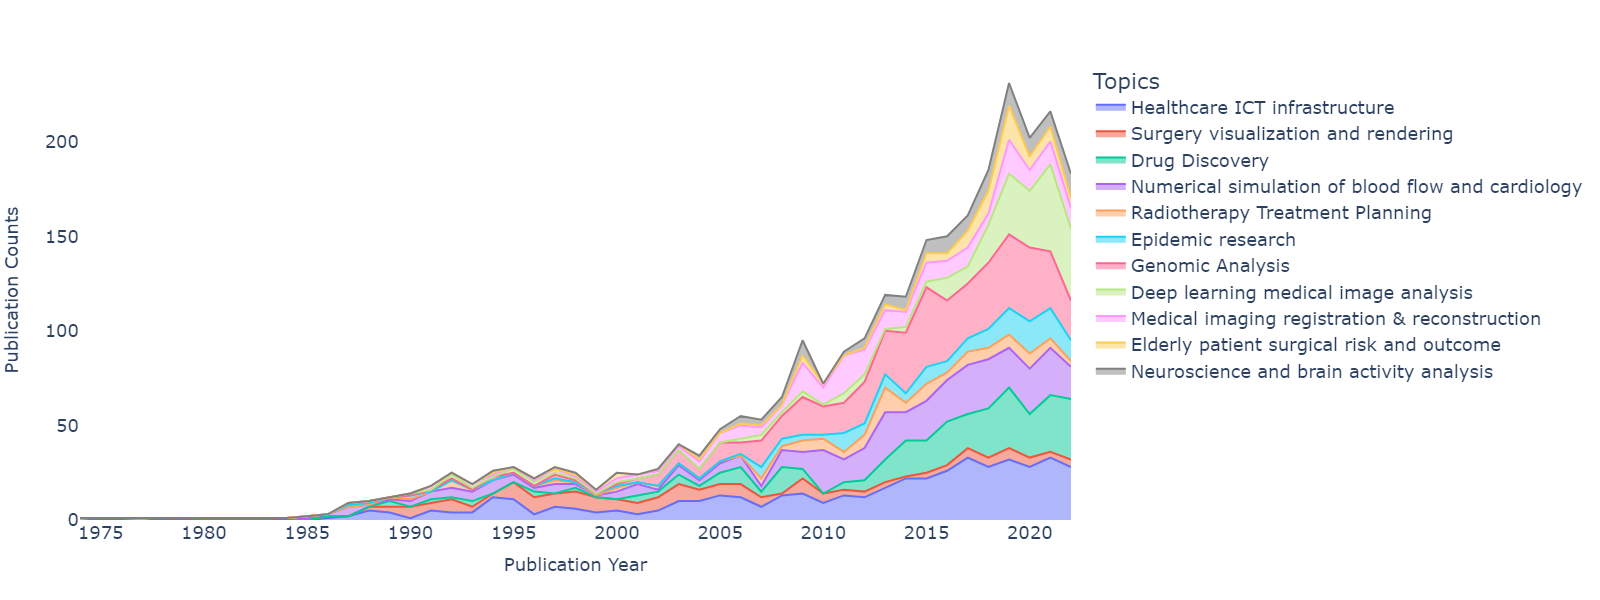
\includegraphics[width=1.0\textwidth]{2-4.png}
\caption{Stacked area chart illustrating trends in HPC adoption in healthcare cross application domains over time. Each segment represents a specific topic. The thickness of segments reflects topic-specific publication volume}
\label{fig:2-4}
\end{figure}

\begin{figure}[!h]
\centering
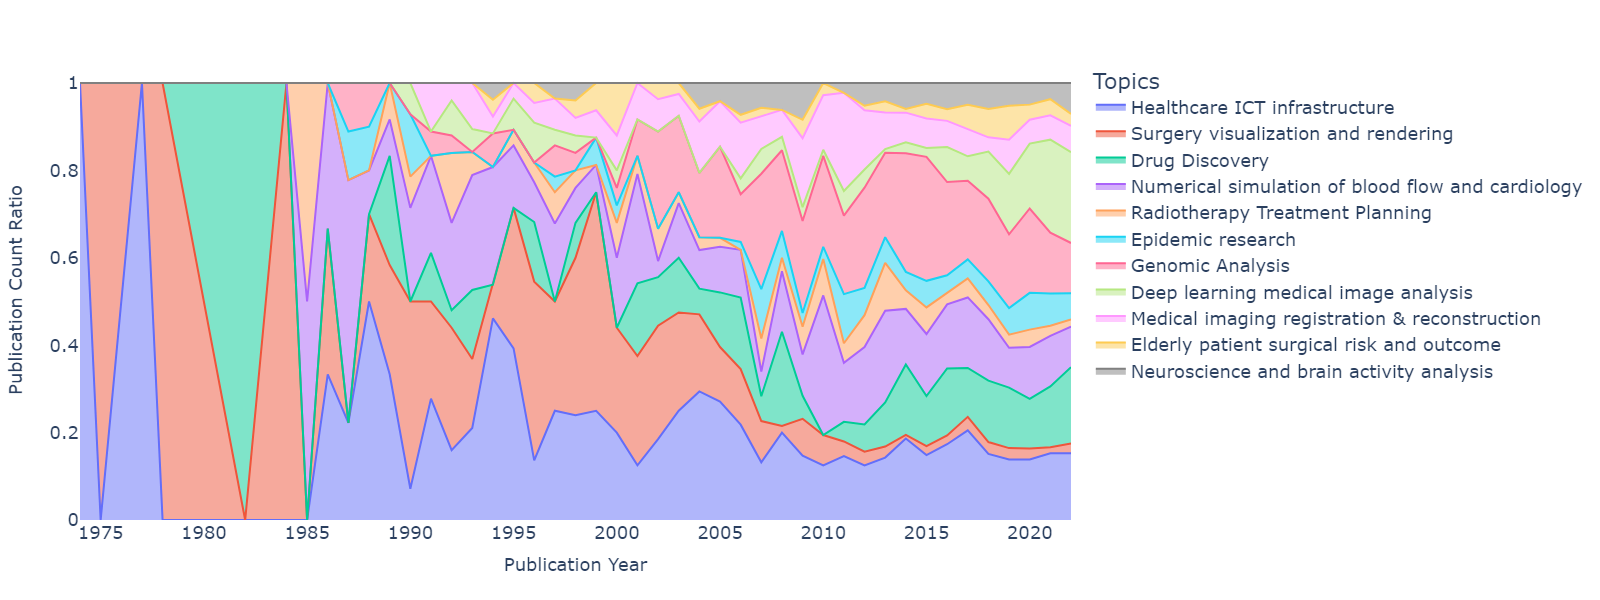
\includegraphics[width=1.0\textwidth]{2-5.png}
\caption{Normalized stacked area chart depicting the relative distribution of HPC adoption in healthcare across application domains over time. Each segment represents a specific topic. The thickness of segments reflects normalized proportion of publication counts}
\label{fig:2-5}
\end{figure}

The violin chart presented in Figure~\ref{fig:2-6} confirms the insights derived from the stacked area chart, specifically the extensive investigation of healthcare ICT infrastructure in the past thirty years. From 2005 onwards, a marked shift has been observed in the utilization of HPC in medical imaging research. Initially, the focus was predominantly on image registration and reconstruction. However, after 2015, there was a significant transition towards the incorporation of deep learning techniques for image analysis. Fluid dynamics simulations of blood flow and cardiology, which adopted HPC relatively early, witnessed a significant surge after 2008. Additionally, visualization and rendering in surgical practice, among the earliest applications of HPC, were hot research topics from 1990 to 2010, although interest has waned since. Moreover, research related to epidemic spreading emerged around 2003, concurrent with the SARS-CoV-1 outbreak in Asia, and experienced a tremendous increase in HPC utilization during the global spread of COVID-19, underscoring HPC's growing importance in managing global health crises. Another noteworthy observation is the rising popularity of research on risk and treatment outcomes for elderly patients since 2019, possibly correlated to pandemic research, given the heightened concern for elderly individuals during this crisis. Additionally, the exploding healthcare expenses and the increasing average age of the global population further underscore this emphasis.
\begin{figure}[!h]
\centering
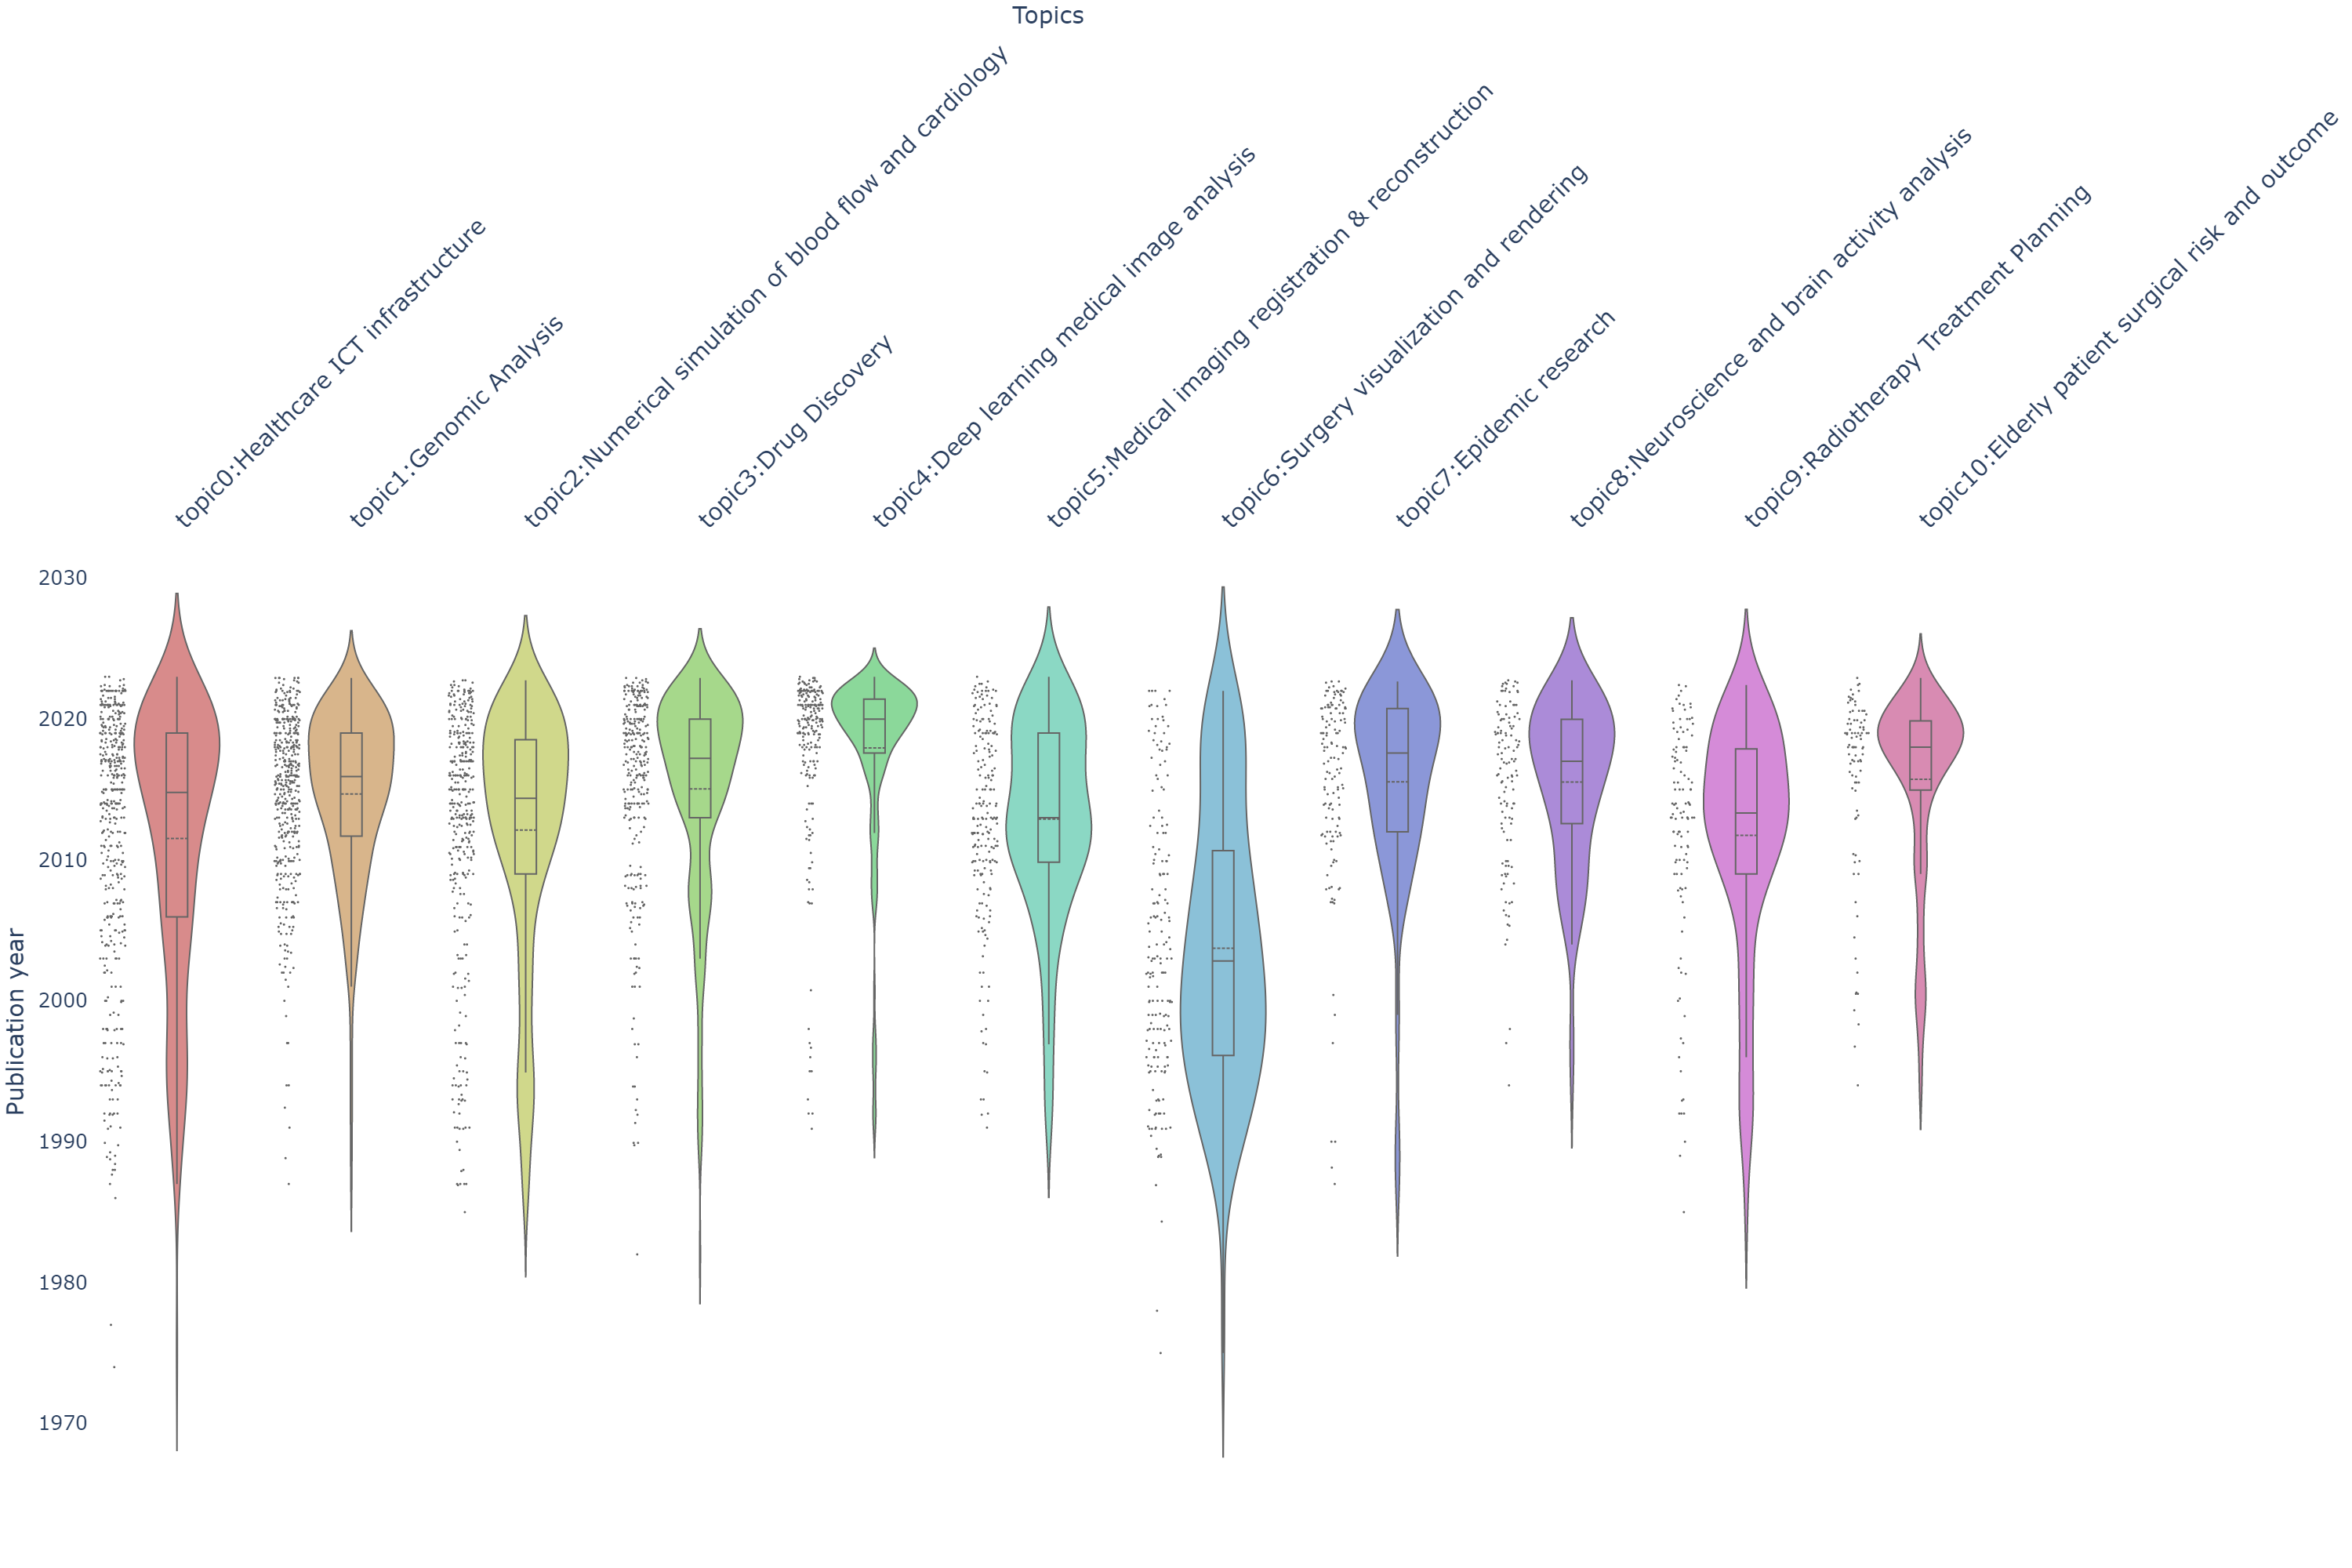
\includegraphics[width=1.0\textwidth]{2-6.png}
\caption{Violin chart depicting the distribution of HPC adoption in healthcare across application domains over time. Violin width represents publication density}
\label{fig:2-6}
\end{figure}

\subsection{Visualizations of topics correlation and convergence}\label{subse:2-3.4}

A bubble chart is constructed using UMAP to visually represent the coverage area of each topic (Figure~\ref{fig:2-7}). Translucent circles were utilized to depict the extent of coverage, while centroid topic vectors are indicated by triangular markers. Additionally, square markers are employed to symbolize the three most-cited papers for each topic. The top six keywords associated with each topic are also presented beneath their respective vectors. All publications form a point cloud, depicted in the background. The chart also incorporates interactive visualization mechanisms: hovering the mouse cursor over each square marker brings up details such as the paper's associated topics, ID, title, citation count, and abstract. This bubble chart provides substantial insights into the correlation and potential convergence trends of the topics, observable through the distances and overlaps between them. As indicated in Figure~\ref{fig:2-7}, a notable observation is the proximity of topics related to deep learning for medical image analysis to neuroscience and brain research. This suggests an extensive application of HPC-enabled medical imaging analysis within neuroscience research. In addition, the research related to simulations of cardiovascular \& blood flow, epidemic research, and drug discovery closely aligns with and overlap the topic of surgical risk and outcomes for elderly patients, indicating a focus on elderly patient outcomes across these topics. Furthermore, by examining the position of highly-cited papers within the bubble chart, we notice that some papers either represent pioneering studies, or span multiple domains, applying specific techniques to innovative fields. For instance, one of the highly cited papers titled `High performance computing for deformable image registration: Towards a new paradigm in adaptive radiotherapy'~\cite{samant2008high} (marked with a black arrow), is located in the intersection area of the topics `medical imaging registration \& reconstruction' and `radiation therapy planning'. This paper highlights the implementation of HPC for near real-time deformable image registration in radiotherapy, indicating that interdisciplinary papers might contribute to greater popularity and citation rates.

\begin{figure}[!h]
\centering
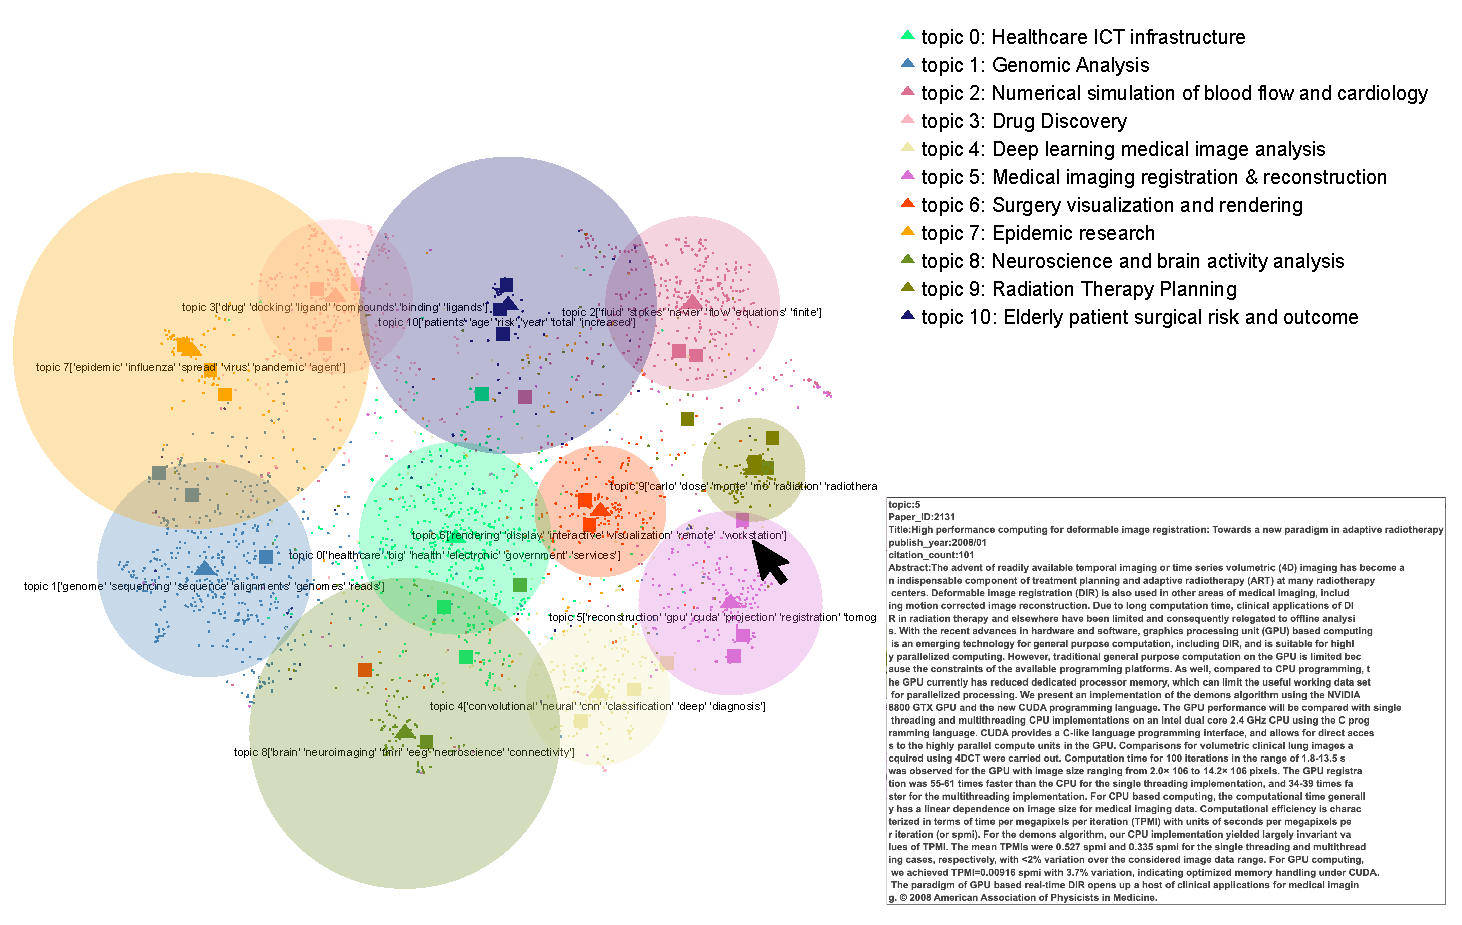
\includegraphics[width=1.0\textwidth]{2-7.pdf}
\caption{Bubble chart showing topic coverage areas based on UMAP. Translucent circles represent each topic's coverage area, centered at the topic's centroid and encompassing 70\% of associated literature. Centroid topic vectors are represented by triangular markers, and the three most-cited papers are indicated with square markers. A text box provides in-depth details on highly cited papers, including associated topics, ID, title, citation count, and abstract}
\label{fig:2-7}
\end{figure}

\section{Identifying future opportunities through analysis of past and present HPC adoption in healthcare}\label{se:2-4}

Historical analysis of HPC adoption within the healthcare sector illustrates a compelling transformation from a specialized technology  into a foundational tool for modern medicine. Originally, HPC was predominantly utilized for complex modeling and biological computations within academic research. However, its role has become more encompassing, opening new and fascinating medical and business opportunities over time. The convergence between simulation and AI, such as neural rendering, seamlessly melds computer graphics and deep learning, opening new avenues in diagnostics and personalized care. Concurrently, the consistent growth in genomics and drug discovery, accelerated by HPC, allows businesses to create dynamic models for pharmaceutical development, reducing cost and time-to-market. In addition, the rise of HPC in global epidemic research presents unique opportunities for developing real-time health monitoring systems, aligning commercial interests with public health needs, and enhancing our response to global health crises. The integration of HPC with emerging technologies such as AI and the Internet of Things (IoT) has further fostered innovative applications in telemedicine and remote monitoring, creating opportunities for healthcare providers to offer services across geographical boundaries. The fusion of technological advancements with unique patient needs has the potential to give birth to virtual care platforms, personalized treatment protocols, or even community-based wellness programs. These innovations align with the growing focus on aging populations, offering a compassionate and tailored approach to healthcare that could become a promising business domain.

The landscape of HPC adoption in healthcare represents an invitation to visionary business thinking, reflecting a future where innovation meets well-being. Collaboration among technology vendors, healthcare institutions, pharmaceutical companies, and startups can leverage the lessons learned from the past and the current state of HPC technology to forge partnerships, develop new products, and create service models that cater to an increasingly interconnected and data-driven healthcare environment. The analytical understanding of this evolution can serve as a guide for future endeavors, nurturing an ecosystem where technological advancement is aligned with healthcare requirements. In this convergence, both sectors stand to gain substantially from sustained cooperation and exploration. More importantly, as regulatory landscapes evolve to embrace technological advancement, it is imperative for stakeholders to understand the historical growth and current trends in HPC adoption in healthcare, as it will guide strategic decision-making and foster further innovation and growth in this interdisciplinary field. 

\section{Discussion}\label{se:2-5}

This study presents an automatic literature analysis framework that utilizes advanced topic modeling techniques (Top2Vec), within the context of the field of HPC adoption in healthcare as the testbed. Through this framework, we effectively process and analyze a substantial volume of scientific literature. The interactive visualizations shed light on the key trends and recognized the emerging research directions in a highly efficient manner. Given that the landscape of HPC adoption in healthcare is extensive and rapidly evolving, the automatic literature analysis offers a scalable and practical approach for researchers and stakeholders to identify trends and potential avenues for future exploration. Continuous tracking of these developments is necessary to maintain a dynamic understanding of the HPC landscape in healthcare, which enables the anticipation of its future.

One of the main limitations of using topic models, such as Top2Vec is the necessity for human intervention to determine the optimal number of topics, which is the only step requiring human input in our otherwise fully automatic literature analysis pipeline. Although metrics such as perplexity and coherence scores can provide guidance towards an optimal topic number, existing literature suggests that these metrics may occasionally be misleading and do not always align with human judgement~\cite{hasan2021normalized,harrando2021apples}. Determining the ideal number of topics within a topic model is a subjective decision that depends on the specific context and goals of the analysis. It requires a balance between having a sufficient number of topics to capture the underlying themes in the data and avoiding excessive fragmentation or overlap between topics. Therefore, human experience and judgment play a critical role in defining the optimal topic count. For this reason, we have integrated the use of a dendrogram to assist in determining the optimal topic count in a more intuitive manner.

Another challenge in using topic modeling is related to semantic understanding. While topic models are highly effective in identifying word and document patterns, they fundamentally lack the ability to understand the meaning of the words. This limitation can lead to topics that are difficult to interpret or exhibit semantic inconsistencies, making manual review and interpretation necessary. One possible approach to tackle this challenge is through EL, which can enhance topic modeling by providing an additional layer of explainability~\cite{dillan2023ldaviewer,10.1145/3126686.3126776}. By linking entities to a knowledge base, EL provides contextual understanding, which refines the interpretability of the topics. It effectively resolves ambiguities where identical names might refer to distinct entities, thereby improving the precision of topic clusters.  Moreover, while topic modeling can significantly aid in analyzing the vast volumes of scientific literature, it cannot replace the critical and contextual understanding that researchers bring to literature review. It should be regarded as a supplementary tool designed to assist in guiding literature exploration rather than serving as an autonomous solution. Given these limitations, future research should strive to fine-tune this methodology, improve the interpretability of the resulting topics, and investigate alternative methods for model evaluation. Despite the inherent challenges, topic modeling remains a potent instrument for managing and comprehending the ever-expanding corpus of scientific literature.

In conclusion, we propose an automatic literature analysis framework which can be easily applied across diverse literature domains, exemplifying its utility through the examination of literature within the field of HPC adoption in healthcare. The insights derived from this study are expected to guide researchers and practitioners toward recognizing emerging opportunities and challenges in the deployment of HPC in healthcare. These findings would contribute to a more informed and strategic incorporation of HPC in healthcare settings, holding the potential to transform medical research and clinical practice in the years to come.





















